% Provenance (never printed): see sources/outline_sources.md (Year 3: gravitational
% potential, spherical harmonics, J2, reference ellipsoid, geoid, satellite gravimetry,
% flexure of the lithosphere). Brief: sources/book5/BRIEFS.md, ch. 3. Curves from
% figdata/bachelor-3/hydrostatic_figure.py, ice_mass.py (IMBIE 2021), flexure.py.
% Exercise and problem values in the Book 5 scratch calculator calc/ch03.py.
\chapter{重力与地球的形状}\label{ch:b3:gravity-geodesy}

两颗卫星一前一后绕地球飞行，轨道高度超过
\qty{500}{km}，彼此相距约\qty{220}{km}，并持续测量二者之间的距离，
精度达到微米量级。
% ledger: geod5:grace, geod5:grace-ranging
当两星经过质量集中的区域时，前方卫星先被拉开，
两星间距随之增大；随后后方卫星被拉近，
间距随之缩小。自 2002 年以来，人们根据这些微小变化，
逐月描绘地球重力场的变化：流域中储存的水随季节涨落，
格陵兰与南极的大型冰盖逐年失去质量。
重力衡量着肉眼看不见的东西。
本章从势出发建立旋转行星的重力场，
由此求得扁率与转动惯量，
把重力异常延伸到轨道高度，再讨论
重力在地表揭示的现象之一：火山重压下岩石圈的弯曲。

\begin{recall}
牛顿万有引力定律、重力势能与
旋转坐标系中的离心力属于物理教材的内容；固体的转动惯量与
勒让德多项式 $P_2(x) = (3x^2 - 1)/2$ 见于物理与数学教材的大学分册；
杨氏模量 $E$ 与
泊松比 $\nu$ 见于物理教材的本科三年级分册。大地测量学与
椭球扁率 $f = (a - b)/a$（半轴 $a > b$）在
十年级已经学过。地壳均衡、艾里补偿、正常重力、大地水准面、
大地水准面高与重力异常，已在本科一年级分册中
关于地壳均衡与重力异常的一章中定义。
\end{recall}

\section{大地位势}

在旋转的行星上，静止的物体既受行星质量的吸引，
在随之转动的坐标系中还受离心力作用。两者都由
势导出。

\begin{definition}[大地位势]\label{def:b3:gravity-geodesy:geopotential}
在随地球以角速度 $\omega$ 旋转的坐标系中，单位质量的势能
即引力势能与离心势能之和，称为
\emph{大地位势}\index{大地位势}：
\[
  W(\mathbf r) = V(\mathbf r) + \Phi(\mathbf r),\qquad
  V(\mathbf r) = -G\int_{\text{Earth}}\frac{\mathrm dm'}{|\mathbf r - \mathbf r'|},\qquad
  \Phi(\mathbf r) = -\tfrac12\omega^2 s^2,
\]
其中 $s$ 为到旋转轴的距离。重力为
$\mathbf g = -\nabla W$，$W = \text{常数}$ 的曲面即为其等位面，
重力处处与等位面垂直。
\end{definition}

铅垂线沿 $-\nabla W$ 方向悬挂，静止的水面则落在等位面上。
因此，旋转的流体行星呈现其自身某一等位面的形状：
离心势在赤道处最深，使赤道隆起，
两极变扁。

\begin{omfigure}
\begin{tikzpicture}[font=\small, x=1cm, y=1cm]
\draw[gray, densely dashed] (0,0) circle (2.4);
\draw[very thick, blue!60!black] (0,0) ellipse (2.75 and 2.1);
\draw[->, thick] (0,-2.7) -- (0,2.9) node[above] {自转轴};
\draw[gray] (-3.2,0) -- (3.2,0);
\fill (0,0) circle (1.6pt);
% a point at latitude 40 deg (parameter) on the ellipse; the attraction points at
% the centre, the centrifugal force is horizontal, and their sum is drawn along the
% inward normal of the ellipse: lengths solved so that the sum is normal (calc/ch03_fig.py)
\coordinate (P) at (2.107,1.350);
\fill (P) circle (1.8pt);
\draw[->, thick, red!70!black] (P) -- (1.012,0.650);
\node[font=\scriptsize, red!70!black, anchor=south east] at (1.50,1.02) {引力};
\draw[->, thick, orange!80!black] (P) -- (2.565,1.350) node[right, font=\scriptsize] {离心力};
\draw[gray, densely dotted] (1.012,0.650) -- (1.470,0.650);
\draw[->, very thick, green!45!black] (P) -- (1.470,0.650);
\node[font=\scriptsize, green!45!black, anchor=north] at (1.470,0.600) {重力};
\node[blue!60!black, anchor=west, font=\scriptsize] at (2.4,-1.7) {等位面};
\node[gray!40!black, anchor=east, font=\scriptsize] at (-1.9,-2.2) {球面};
\end{tikzpicture}

\par\smallskip{\small 旋转行星的等位面（示意图，扁率大为夸大）。
在每一点，重力为引力与离心力之和，
它与等位面处处垂直，除两极和赤道外，
重力并不指向球心。}
\label{fig:b3:gravity-geodesy:equipotential}
\end{omfigure}

在行星外部，引力势满足拉普拉斯方程，
其在无穷远处正则的解即为实球谐函数。

\begin{proposition}[大地位势的球谐展开]\label{prop:b3:gravity-geodesy:harmonics}
设质量为 $M$、赤道半径为 $a$ 的天体，
原点取在质心，$z$ 轴沿自转轴，则其外部
距离为 $r$、余纬为 $\theta$、经度为 $\lambda$ 处的引力势为
\begin{multline*}
  V = -\frac{GM}{r}\Biggl[1 - \sum_{n=2}^{\infty}\left(\frac ar\right)^nJ_nP_n(\cos\theta)\\
  + \sum_{n=2}^{\infty}\sum_{m=1}^{n}\left(\frac ar\right)^nP_{nm}(\cos\theta)
  (C_{nm}\cos m\lambda + S_{nm}\sin m\lambda)\Biggr],
\end{multline*}
其中 $P_n$ 为勒让德多项式，$P_{nm}$ 为连带勒让德函数；
系数 $J_n$、$C_{nm}$、$S_{nm}$ 为由观测拟合得到的数值。对于绕轴对称的天体，
只剩下带谐项 $J_n$。展开式中
不含度为 1 的项。
\end{proposition}

\begin{proof}
在球坐标中对拉普拉斯方程分离变量，
得到无穷远处正则的解 $r^{-(n+1)}P_{nm}(\cos\theta)e^{\pm
im\lambda}$（见数学教材的大学分册）；质量分布之外的任意势
都是这些解之和。零次项为 $-GM/r$，
即整个质量的势。一次项正比于一阶矩
$\int\mathbf r'\,\mathrm dm'$，当原点取在质心时它为零。
轴对称性去掉了所有依赖于 $\lambda$ 的项。
\end{proof}

\begin{definition}[动力学形状因子]\label{def:b3:gravity-geodesy:j2}
行星的\emph{动力学形状因子}\index{动力学形状因子} $J_2$ 是其
二阶纬向谐波的系数，即其外部势相对于球体的最大偏离，
由扁率引起。对于
地球，$J_2 = \num{1.08263e-3}$。
% ledger: geod5:grs80-defining
\end{definition}

\begin{theorem}[麦卡拉公式]\label{thm:b3:gravity-geodesy:maccullagh}
设 $A$、$B$、$C$ 为质量为 $M$ 的物体关于过其质心的坐标轴的
主转动惯量，$I$ 为其关于从质心到外部一点连线的转动惯量，
该外部点与质心的距离为 $r$。
在 $r^{-3}$ 阶精度下，该点的引力势由
\emph{麦卡拉公式}\index{麦卡拉公式}给出：
\[
  V = -\frac{GM}{r} - \frac{G(A + B + C - 3I)}{2r^3} .
\]
对于关于 $z$ 轴对称的物体（$A = B$），
$V = -\dfrac{GM}{r} + \dfrac{G(C - A)}{r^3}P_2(\cos\theta)$，于是
\[
  J_2 = \frac{C - A}{Ma^2} .
\]
\end{theorem}

\begin{proof}
设 $\hat{\mathbf r}$ 为指向该点的单位矢量，$r' \ll r$，则
\[
  \frac{1}{|\mathbf r - \mathbf r'|} = \frac1r + \frac{\hat{\mathbf r}\cdot\mathbf r'}{r^2}
  + \frac{3(\hat{\mathbf r}\cdot\mathbf r')^2 - r'^2}{2r^3} + O(r^{-4}).
\]
对质量积分，第一项给出 $M/r$，第二项为零
（质心）。对第三项，$\int r'^2\,\mathrm dm' = (A + B + C)/2$，因为
$A + B + C = \int 2r'^2\,\mathrm dm'$，且 $\int(\hat{\mathbf r}\cdot\mathbf
r')^2\,\mathrm dm' = \int r'^2\,\mathrm dm' - I$，
而到该连线的距离平方为 $r'^2 - (\hat{\mathbf r}\cdot\mathbf r')^2$。括号内的积分为
$3(A + B + C)/2 - 3I - (A + B + C)/2 = A + B + C - 3I$。对于 $A = B$，
关于余纬为 $\theta$ 的直线的转动惯量为 $I = A\sin^2\theta + C\cos^2\theta$，
且 $2A + C - 3I = (C - A)(1 - 3\cos^2\theta) = -2(C - A)P_2(\cos\theta)$。
与\cref{prop:b3:gravity-geodesy:harmonics}比较可得
$J_2Ma^2 = C - A$。
\end{proof}

因此，势的二阶项度量的是
转动惯量之差，而非转动惯量本身。地球自转轴的岁差
由太阳和月球作用于赤道隆起的力矩驱动，
度量动力学椭率 $H = (C - A)/C$；将 $J_2$ 与 $H$ 结合，
得到 $C/(Ma^2)$，即转动惯量因子，地球的该值为 \num{0.3308}，
% ledger: earth:MoI
远小于均匀球体的 \num{0.4}：质量向
地心集中。

\section{旋转椭球}

\begin{definition}[参考椭球]\label{def:b3:gravity-geodesy:ellipsoid}
称\emph{参考椭球}\index{参考椭球}为一旋转椭球体，
其赤道半轴为 $a$、扁率为 $f$，选取时使之
本身为某一模型势的等势面，该模型势即
质量为 $M$、角速度为 $\omega$ 的旋转物体的势，其中的\omterm{def:b3:gravity-geodesy:j2}{动力学形状
因子}取地球的 $J_2$。四个常数确定它，1980 年大地参考
系统取
\begin{gather*}
  a = \qty{6378137}{m},\qquad GM = \qty{3.986005e14}{m^3.s^{-2}},\\
  J_2 = \num{1.08263e-3},\qquad \omega = \qty{7.292115e-5}{rad.s^{-1}},
\end{gather*}
并由此导出扁率 $f = \num{0.00335281068}$，
（$1/f = \num{298.257222}$），以及短半轴
$b = \qty{6356752.3141}{m}$.
% ledger: geod5:grs80-defining, geod5:grs80-derived
\end{definition}

模型的势，即正常势，可写成闭式，
其在椭球面上的重力亦然，即本科一年级分册中的正常重力。

\begin{proposition}[索米利亚纳公式]\label{prop:b3:gravity-geodesy:somigliana}
设\omterm{def:b3:gravity-geodesy:ellipsoid}{参考椭球}的半轴为 $a$、$b$，其正常重力
在赤道处为 $\gamma_e$，在两极处为 $\gamma_p$，则
大地纬度 $\varphi$ 处的正常重力由\emph{索米利亚纳
公式}\index{索米利亚纳公式}给出：
\[
  \gamma(\varphi) = \frac{a\gamma_e\cos^2\varphi + b\gamma_p\sin^2\varphi}
  {\sqrt{a^2\cos^2\varphi + b^2\sin^2\varphi}} .
\]
对于 1980 年大地参考系统，$\gamma_e = \qty{9.7803267715}{m.s^{-2}}$，
$\gamma_p = \qty{9.8321863685}{m.s^{-2}}$，并有级数
$\gamma = 9.780327(1 + 0.0053024\sin^2\varphi - 0.0000058\sin^22\varphi)$
\unit{m.s^{-2}}，与该公式的符合精度达 \qty{0.1}{\milli\gal}。
% ledger: geod5:grs80-derived, moritz:grs80 (Book 3, read-only)
\end{proposition}
\admitted

旋转行星应有多扁？若它是处于静力
平衡的流体，其扁率由自转以及
质量沿深度的分布所决定。

\begin{proposition}[克莱罗与达尔文–拉多关系]\label{prop:b3:gravity-geodesy:clairaut}
对于处于静力平衡的行星，记 $m = \omega^2a^2b/(GM)$ 为
赤道处离心加速度与引力加速度之比，准确到
$f$ 与 $m$ 的一阶：
\[
  J_2 = \frac{2f - m}{3}\qquad\text{（克莱罗）},\qquad
  \frac{C}{Ma^2} = \frac23\left[1 - \frac25\sqrt{\frac52\frac mf - 1}\right]
  \qquad\text{（达尔文–拉多）} .
\]
均匀行星（$C/Ma^2 = 0.4$）满足 $f = 5m/4$；质量
集中于中心附近的行星扁率更小。
\end{proposition}
\admitted

由克莱罗关系，取地球的 $m = \num{0.00344979}$，将其实测的
$J_2$ 换算为 $f = \num{0.0033488}$，即 $1/298.6$，与椭球的
扁率相差在 \qty{0.12}{\percent} 以内。达尔文–拉多
关系结合转动惯量因子，给出地球若为平衡流体时应有的扁率，
即 $1/299.9$，而实测值为
$1/298.26$。地球比自转与质量分布相同的流体行星略扁，
其赤道隆起比静力平衡所预言的高出约
\qty{116}{m}。地球并非严格处于平衡的流体，
这一微小差异本身，
便是对其内部所承受应力的一种度量。

\begin{omfigure}
\begin{tikzpicture}
\begin{axis}[omrecord, width=0.74\linewidth, height=0.44\linewidth,
  xmin=0.3, xmax=0.4, ymin=225, ymax=340,
  xlabel={转动惯量因子 $C/(Ma^2)$}, ylabel={静力平衡 $1/f$},
  xtick={0.30,0.32,0.34,0.36,0.38,0.40},
  xticklabel style={/pgf/number format/fixed, /pgf/number format/precision=2}]
\addplot[blue!70!black, thick] table[x=moi, y=f_inv] {figdata/out/bachelor-3-hydrostatic_figure-curve.dat};
\draw[gray, densely dashed] (axis cs:0.3308,225) -- (axis cs:0.3308,299.88);
\draw[gray, densely dashed] (axis cs:0.3,299.88) -- (axis cs:0.3308,299.88);
\fill[blue!70!black] (axis cs:0.3308,299.88) circle (2pt);
\node[font=\scriptsize, anchor=south west] at (axis cs:0.3315,301) {静力平衡地球，$1/f = 299.9$};
\draw[red!70!black, thick] (axis cs:0.3,298.26) -- (axis cs:0.4,298.26);
\node[font=\scriptsize, anchor=north east, red!70!black] at (axis cs:0.399,296.5) {实测，$1/f = 298.26$};
\fill (axis cs:0.4,231.9) circle (2pt);
\node[font=\scriptsize, anchor=east] at (axis cs:0.397,233) {均匀行星};
\end{axis}
\end{tikzpicture}

\par\smallskip{\small 取地球自转速率时，流体行星的扁率
随其转动惯量因子的变化，由达尔文–拉多关系式得出
（按 1980 年大地参考系统计算）。质量越
集中于中心，行星越圆。在地球的
\num{0.3308} 处，静力平衡扁率为 $1/299.9$，略小于
实测的 $1/298.26$。}
\label{fig:b3:gravity-geodesy:hydrostatic}
\end{omfigure}

\section{大地水准面与扰动位}

大地水准面是与平均海平面重合的真实\omterm{def:b3:gravity-geodesy:geopotential}{位势}的等位面；
\omterm{def:b3:gravity-geodesy:ellipsoid}{参考椭球}是正常位 $U$ 的一个等位面，
其值与之相同，$U_0 = W_0$。二者的间距即大地水准面高 $N$，
由两个位的差决定。

\begin{proposition}[布伦斯公式]\label{prop:b3:gravity-geodesy:bruns}
设 $T = W - U$ 为扰动位。某点处的大地水准面高
由\emph{布伦斯公式}\index{布伦斯公式}给出
\[
  N = -\frac{T}{\gamma},
\]
其中 $T$ 取在大地水准面上的值，$\gamma$ 为该处的正常重力。
质量盈余使位降低（$T < 0$），抬高大地水准面。
\end{proposition}

\begin{proof}
设 P 为大地水准面上的点，Q 为椭球上位于其下方、距离为
$N$ 的点。由于 $U$ 向外以速率 $\gamma$ 增大，
$U(\mathrm P) = U(\mathrm Q) + \gamma N = U_0 + \gamma N$。于是
$W_0 = W(\mathrm P) = U(\mathrm P) + T(\mathrm P) = U_0 + \gamma N + T$，且
由 $W_0 = U_0$ 得 $N = -T/\gamma$。
\end{proof}

大地水准面高为 \qty{50}{m} 时，对应的位差仅为
\qty{490}{J.kg^{-1}}，约为\omterm{def:b3:gravity-geodesy:geopotential}{位势}的 \num{e5} 分之一。地球的大地水准面高
从冰岛附近的约 $+\qty{85}{m}$，到
印度南部的 $-\qty{106}{m}$，
% ledger: nasa:geoid-range (Book 3, read-only)
这一变化范围不足 \qty{200}{m}，而地球的赤道半径与极半径
相差 \qty{21}{km}。

\section{卫星重力测量}

\begin{definition}[卫星重力测量]\label{def:b3:gravity-geodesy:satgrav}
\emph{卫星重力测量}\index{卫星重力测量}利用卫星的运动确定地球的
重力场：由卫星轨道的长期摄动，
由同轨两颗卫星间距离的变化，
或由梯度仪测量
航天器两端的重力差。
\end{definition}

近地轨道受到的最大摄动来自 $J_2$。赤道隆起
对倾斜轨道施加力矩，使轨道面
绕地轴缓慢转动。

\begin{proposition}[节点进动]\label{prop:b3:gravity-geodesy:nodal}
在 $J_2$ 的一阶近似下，半径为 $r$、倾角为 $i$ 的圆轨道，其节线
以如下速率转动：
\[
  \dot\Omega = -\frac32\,nJ_2\left(\frac ar\right)^2\cos i,\qquad n = \sqrt{GM/r^3} ,
\]
对顺行轨道（$i < \ang{90}$）向西，对逆行轨道向东。
\end{proposition}

\begin{proof}
经过许多圈运行后，卫星的作用相当于沿
轨道分布、质量为 $m_s$ 的环。\omterm{def:b3:gravity-geodesy:geopotential}{位势}的二阶部分
$(GMJ_2a^2/r^3)P_2(\cos\theta)$（单位质量），在倾角为
$i$ 的圆上取平均，涉及 $\langle\cos^2\theta\rangle = \tfrac12\sin^2i$，故
$\langle P_2\rangle = \tfrac34\sin^2i - \tfrac12$，环的能量为
$E(i) = m_s(GMJ_2a^2/r^3)(\tfrac34\sin^2i - \tfrac12)$。绕节线的
力矩为 $\tau = -\mathrm dE/\mathrm di = -\tfrac32m_s(GMJ_2a^2/r^3)\sin
i\cos i$。它垂直于环的角动量 $L = m_snr^2$，因此
使 $\mathbf L$ 绕极轴转动而其长度不变：
$L\sin i\,\dot\Omega = \tau$。由 $GM = n^2r^3$，得 $\dot\Omega =
-\tfrac32nJ_2(a/r)^2\cos i$。
\end{proof}

对位于赤道附近的低轨卫星，该速率每天可达数度；在
倾角略大于 \ang{90} 时，它恰与太阳的周年运动相吻合，轨道
全年相对太阳保持同一取向（见练习 12）。对许多倾角不同的卫星进行测量，
这类进动可给出 $J_2$ 及
更高阶的带谐项。

一对卫星效果更好：二者之间距离的变化，测得的是
它们沿轨道所感受到的重力差。GRACE 双星于 2002 年至 2017 年运行，其后继星
GRACE Follow-On 自 2018 年 5 月 22 日发射以来运行，其微波链路
可将距离测量到微米量级，激光链路用以检验，
精度可提高至二十倍。
% ledger: geod5:grace, geod5:grace-ranging
地球重力场逐月变化，原因在于水的迁移：积雪与土壤湿度、
地下水、湖泊、海洋与冰盖。

\begin{omfigure}
\begin{tikzpicture}[font=\small, x=1cm, y=1cm]
\draw[thick, brown!60!black] (-5,0) -- (1.6,0) .. controls (2.0,0.08) and (3.0,0.08) .. (3.4,0) -- (5,0);
\fill[blue!25] (1.8,0) rectangle (3.2,-0.6);
\node[font=\scriptsize] at (2.5,-0.3) {质量盈余};
\draw[gray, densely dashed] (-5,2.5) -- (5,2.5);
\node[gray!40!black, font=\scriptsize, anchor=south west] at (-5,2.55) {轨道};
\fill[orange!80!black] (-2.6,2.35) rectangle (-2.0,2.65);
\fill[orange!80!black] (0.4,2.35) rectangle (1.0,2.65);
\draw[<->, red!70!black, thick] (-1.95,2.5) -- (0.35,2.5) node[midway, above, font=\scriptsize] {距离，约 \qty{220}{km}};
\draw[->, thick] (0.85,2.3) -- (1.45,1.75);
\draw[->, thick, gray] (2.6,2.9) -- (4.2,2.9) node[right, font=\scriptsize] {运动};
\node[font=\scriptsize, anchor=north, align=center] at (0.2,1.6) {前导卫星先被拉向前，\\距离增大};
\node[font=\scriptsize, anchor=north, align=center] at (-2.9,1.6) {随后后随卫星也被拉向前，\\距离减小};
\end{tikzpicture}

\par\smallskip{\small 卫星对原理示意图（非按比例绘制）。
接近质量盈余时，前导卫星先受其吸引，
并向前加速，因此两星之间的距离增大；
当后随卫星经过该质量上方时，距离又减小。
距离变化率经连续测量，据此反演重力场。}
\label{fig:b3:gravity-geodesy:grace}
\end{omfigure}

\begin{omfigure}
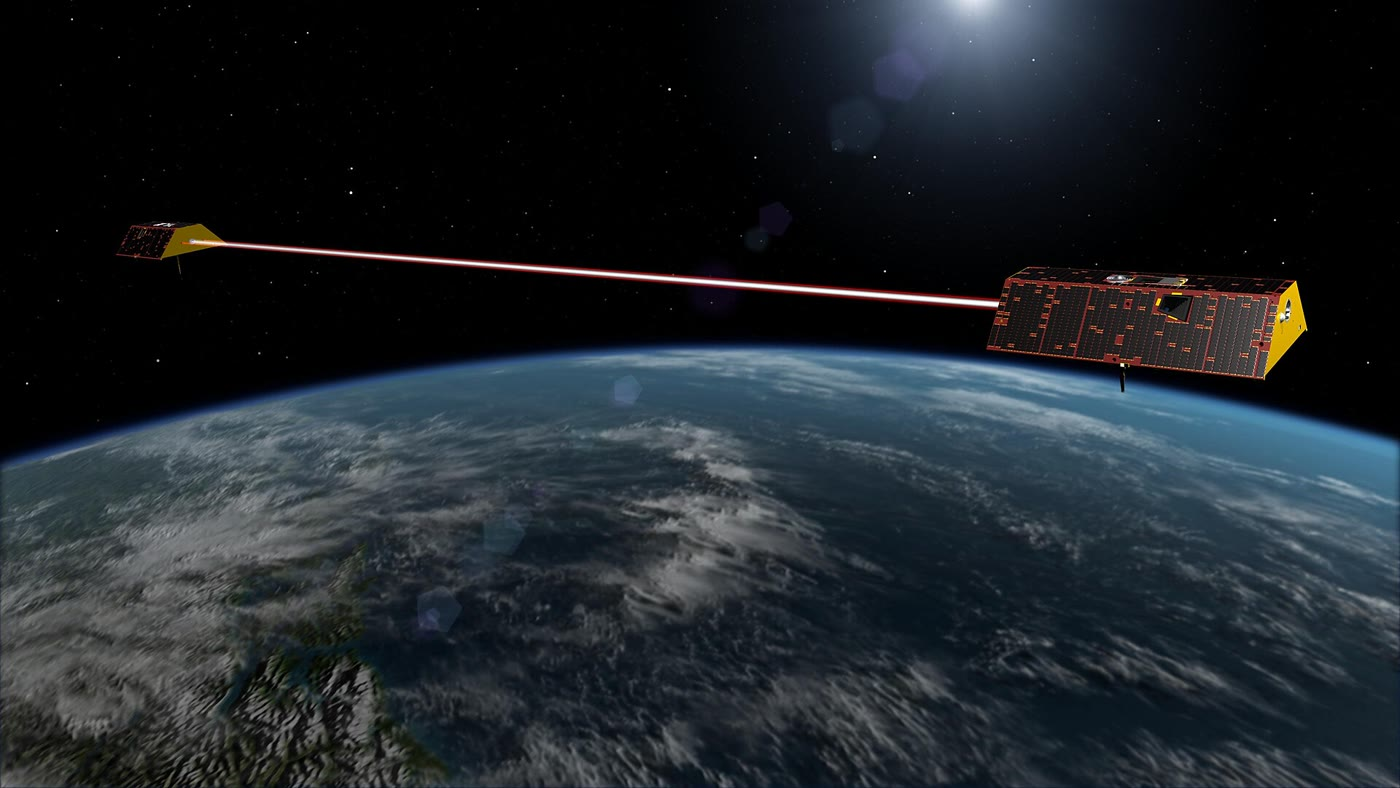
\includegraphics[width=0.66\linewidth]{images/book5/b3-grace-fo-concept.jpg}

\par\smallskip{\small GRACE Follow-On 双星的艺术家构想图（
两星之间的距离被大幅缩短）。红色光束表示激光
测距链路。NASA/JPL-Caltech，公有领域。}
\label{fig:b3:gravity-geodesy:grace-photo}
\end{omfigure}

\begin{definition}[等效水高]\label{def:b3:gravity-geodesy:ewh}
若重力场的变化在远大于质量迁移所在层厚度的距离上缓慢变化，
则可用地表一个薄壳上的面密度
变化 $\sigma$（\unit{kg.m^{-2}}）来表示。
\emph{等效水高}\index{等效水高}
是指面密度与之相同的淡水厚度：
\[
  h_w = \frac{\sigma}{\rho_w} .
\]
\end{definition}

在面积为 \qty{1e6}{km^2} 的流域上，一米厚的水的质量为 \qty{1e15}{kg}，或
\qty{1000}{Gt}。海平面则是账本的另一面：\qty{360}{Gt} 的冰
加入海洋，会使海平面升高约一毫米。
% ledger: data:b5-imbie
\omterm{def:b3:gravity-geodesy:satgrav}{卫星重力测量}、卫星测高，以及降雪量与冰流出量之差，
三者各自测定冰盖的质量平衡；加以综合，
即得到下面的时间序列。

\begin{omfigure}
\begin{tikzpicture}
\begin{axis}[omrecord, width=0.82\linewidth, height=0.5\linewidth,
  xmin=1992, xmax=2021, ymin=-5600, ymax=600,
  xlabel={年}, ylabel={累积质量变化（\unit{Gt}）},
  xticklabel style={/pgf/number format/1000 sep={}},
  legend pos=south west, legend cell align=left, legend style={font=\scriptsize}]
\addplot[name path=gl, draw=none, forget plot] table[x=year, y=lo] {figdata/out/bachelor-3-ice_mass-greenland.dat};
\addplot[name path=gh, draw=none, forget plot] table[x=year, y=hi] {figdata/out/bachelor-3-ice_mass-greenland.dat};
\addplot[blue!25, forget plot] fill between[of=gl and gh];
\addplot[name path=al, draw=none, forget plot] table[x=year, y=lo] {figdata/out/bachelor-3-ice_mass-antarctica.dat};
\addplot[name path=ah, draw=none, forget plot] table[x=year, y=hi] {figdata/out/bachelor-3-ice_mass-antarctica.dat};
\addplot[red!20, forget plot] fill between[of=al and ah];
\addplot[blue!70!black, thick] table[x=year, y=cum] {figdata/out/bachelor-3-ice_mass-greenland.dat};
\addlegendentry{格陵兰}
\addplot[red!70!black, thick] table[x=year, y=cum] {figdata/out/bachelor-3-ice_mass-antarctica.dat};
\addlegendentry{南极}
\draw[gray, densely dotted] (axis cs:2002.25,-5600) -- (axis cs:2002.25,600);
\draw[gray, densely dotted] (axis cs:2017.5,-5600) -- (axis cs:2017.5,600);
\node[font=\scriptsize, gray!40!black, anchor=north] at (axis cs:2009.9,550) {GRACE 时段};
\end{axis}
\end{tikzpicture}

\par\smallskip{\small 格陵兰和南极冰盖的累积质量变化，
自 1992 年以来，附一个标准差范围（IMBIE 2021 
综合估计，来自测高、重力测量和输入–输出法）。截至
2020 年底，格陵兰失去了 $\num{4890} \pm \qty{460}{Gt}$，南极
失去了 $\num{2670} \pm \qty{530}{Gt}$；直线拟合给出
1992--2020 年间的变化率分别为 \qty{-176}{Gt.\text{年}^{-1}} 和 \qty{-91}{Gt.\text{年}^{-1}}，
在 GRACE 时段内则分别为 \qty{-246}{Gt.\text{年}^{-1}} 和 \qty{-127}{Gt.\text{年}^{-1}}。}
\label{fig:b3:gravity-geodesy:ice-mass}
\end{omfigure}

地表测得的重力异常是若干谐波之和；在
卫星高度上，每一谐波都会被一个与其
波长有关的因子减弱。

\begin{proposition}[向上延拓]\label{prop:b3:gravity-geodesy:upward}
在产生该异常的质量上方，沿地表按
$\Delta g_0\cos kx$（其中 $k = 2\pi/\lambda$）变化的重力异常，在高度 $z$ 处
的值（即其\emph{向上延拓}\index{向上延拓}）为
\[
  \Delta g(x, z) = \Delta g_0\,e^{-kz}\cos kx .
\]
\end{proposition}

\begin{proof}
在质量上方，异常位及由其导出的异常，
满足拉普拉斯方程 $\partial_x^2\Delta g + \partial_z^2\Delta g = 0$。分离
变量，令 $\Delta g = Z(z)\cos kx$，则 $Z'' = k^2Z$，其在 $z \to \infty$ 时有界的
解为 $Z = \Delta g_0e^{-kz}$。
\end{proof}

在 \qty{400}{km} 高度上，长 \qty{1000}{km} 的异常保留其
振幅的 \qty{8}{\percent}，长 \qty{100}{km} 的异常则仅保留约 \num{1e-11}：
卫星能够探测长波，地表测量则更适合短波。

\section{岩石圈挠曲}

本科一年级分册中的补偿是局地的，每一列各自漂浮。
洋壳板块上的火山并不只在自身之下得到补偿：
板块在其下弯曲，弯曲范围宽达数百千米，火山周围的海底因而下沉，
形成一条洼槽，槽外则以低矮的拱形抬升。

\begin{definition}[岩石圈挠曲、挠曲刚度、有效弹性厚度]\label{def:b3:gravity-geodesy:flexure}
\emph{岩石圈挠曲}\index{岩石圈挠曲}是岩石圈在载荷作用下的弯曲，
可建模为薄弹性板在流体地幔上漂浮时的弯曲。
板抵抗弯曲的能力为
\emph{挠曲刚度}\index{挠曲刚度}，
\[
  D = \frac{ET_e^3}{12(1 - \nu^2)},
\]
而与真实岩石圈弯曲方式相同的均匀弹性板的厚度 $T_e$，
称为其\emph{有效弹性厚度}\index{有效弹性厚度}。
\end{definition}

\begin{theorem}[薄板挠曲]\label{thm:b3:gravity-geodesy:plate}
设刚度为 $D$ 的薄弹性板沿一个方向受单位面积上的载荷 $q(x)$ 作用而弯曲，
向下挠度为 $w(x)$，漂浮于密度为 $\rho_m$ 的地幔之上，
凹陷处充以密度为 $\rho_i$ 的物质，则其满足
\emph{挠曲方程}\index{挠曲方程}
\[
  D\frac{\mathrm d^4w}{\mathrm dx^4} + (\rho_m - \rho_i)g\,w = q(x) .
\]
\end{theorem}

\begin{proof}
弯曲的板中，中面以上的纤维缩短，中面以下的纤维伸长，
其变形量与曲率 $w''$ 成正比；将弯曲应力沿厚度积分，
得弯矩 $M = -Dw''$，其中刚度取定义中的形式
（板不能横向膨胀，故有因子
$1 - \nu^2$；此内容见物理系列本科三年级分册）。板的一个微元 $\mathrm dx$
在其两侧面承受剪力 $V$ 与弯矩 $M$。竖直方向受力平衡：
向下的载荷 $q\,\mathrm dx$ 与被排开地幔向上的浮力
$(\rho_m - \rho_i)gw\,\mathrm dx$ 向上，二者平衡，给出 $\mathrm dV/\mathrm dx = -q +
(\rho_m - \rho_i)gw$。力矩平衡给出 $\mathrm dM/\mathrm dx = V$。
于是 $-Dw'''' = M'' = V' = -q + (\rho_m - \rho_i)gw$。
\end{proof}

\begin{definition}[挠曲参数、前缘隆起]\label{def:b3:gravity-geodesy:alpha}
板的\emph{挠曲参数}\index{挠曲参数}是
长度
\[
  \alpha = \left(\frac{4D}{(\rho_m - \rho_i)g}\right)^{1/4},
\]
它决定了板挠曲的水平尺度。\emph{前缘隆起}\index{前缘隆起}
是弯曲的板在载荷一侧的洼槽或盆地之外
抬起的向上挠曲低拱。
\end{definition}

\begin{proposition}[连续板上的线载荷]\label{prop:b3:gravity-geodesy:line}
单位长度载荷为 $V_0$ 的线载荷作用于 $x = 0$ 处，使板产生挠度
\[
  w(x) = w_0e^{-|x|/\alpha}\left(\cos\frac{|x|}{\alpha} + \sin\frac{|x|}{\alpha}\right),
  \qquad w_0 = \frac{V_0\alpha^3}{8D} .
\]
挠度在 $|x| = 3\pi\alpha/4$ 处为零，即洼槽的边缘；
\omterm{def:b3:gravity-geodesy:alpha}{前缘隆起}的峰顶位于 $|x| = \pi\alpha$ 处，其高度为 $w_0e^{-\pi} =
\num{0.0432}\,w_0$。整个挠曲所受的浮力与载荷平衡：
$\int(\rho_m - \rho_i)gw\,\mathrm dx = V_0$。
\end{proposition}

\begin{proof}
当 $x > 0$ 时方程为 $w'''' + 4w/\alpha^4 = 0$；
$r^4 = -4/\alpha^4$ 的根为 $(\pm1 \pm i)/\alpha$，在远处趋于零的
解为 $e^{-x/\alpha}(A\cos(x/\alpha) + B\sin(x/\alpha))$。对称性要求
$w'(0) = 0$，由此得 $A = B = w_0$。对载荷两侧的竖直平衡积分，
剪力 $V = -Dw'''$ 跳变 $-V_0$；由对称性
$w'''(0^-) = -w'''(0^+)$，且 $w'''(0^+) = 4w_0/\alpha^3$，故 $8Dw_0/\alpha^3 =
V_0$。挠度在 $\tan(x/\alpha) =
-1$ 处为零，首个零点为 $x = 3\pi\alpha/4$；其导数
$-(2w_0/\alpha)e^{-x/\alpha}\sin(x/\alpha)$ 的下一个零点为 $x = \pi\alpha$。
最后，$\int_0^\infty e^{-u}(\cos u + \sin u)\,\mathrm du = 1$，因此
$\int w\,\mathrm dx = 2w_0\alpha = V_0\alpha^4/(4D) = V_0/((\rho_m - \rho_i)g)$。
\end{proof}

\begin{proposition}[断裂板]\label{prop:b3:gravity-geodesy:broken}
板在 $x = 0$ 处断裂，自由端受压向下，如深海海沟处的情形，
则挠度为 $w = w_0e^{-x/\alpha}\cos(x/\alpha)$，
当 $x \ge 0$ 时，挠度在 $x = \pi\alpha/2$ 处为零，
\omterm{def:b3:gravity-geodesy:alpha}{前缘隆起}的峰顶，即外隆起，位于 $x = 3\pi\alpha/4$ 处，其高度为 $w_0e^{-3\pi/4}/\sqrt2 =
\num{0.067}\,w_0$。
\end{proposition}

\begin{proof}
衰减解与前相同，此时自由端不承受弯矩，
$w''(0) = 0$，由此得 $B = 0$。零点位于 $\cos(x/\alpha) = 0$；其导数
$-(w_0/\alpha)e^{-x/\alpha}(\cos + \sin)(x/\alpha)$ 在
$x = 3\pi\alpha/4$ 处为零，此处 $w = w_0e^{-3\pi/4}\cos(3\pi/4)$。
\end{proof}

因此，距离是判断板强度的关键：测出洼槽在何处结束，
或隆起峰顶在何处，即可求得 $\alpha$，进而求得 $D$，再求得 $T_e$。
由于 $T_e$ 以 $\alpha^{4/3}$ 的形式进入，距离的合理估计
即可给出厚度的良好估计。

\begin{omfigure}
\begin{tikzpicture}
\begin{groupplot}[group style={group size=1 by 2, vertical sep=1.5cm},
  width=0.82\linewidth, height=0.36\linewidth, xmin=-400, xmax=400,
  tick label style={font=\scriptsize}, label style={font=\small}, title style={font=\small}]
\nextgroupplot[title={(a) 线载荷：三种厚度板上的 Oru 山脊},
  ylabel={挠度 (\unit{m})}, ymin=-3000, ymax=700, y filter/.expression={-y},
  legend pos=south east, legend cell align=left, legend style={font=\scriptsize}]
\addplot[red!70!black, thick] table[x=x, y=w10] {figdata/out/bachelor-3-flexure-profiles.dat};
\addlegendentry{$T_e = \qty{10}{km}$}
\addplot[blue!70!black, thick] table[x=x, y=w25] {figdata/out/bachelor-3-flexure-profiles.dat};
\addlegendentry{$T_e = \qty{25}{km}$}
\addplot[green!45!black, thick] table[x=x, y=w40] {figdata/out/bachelor-3-flexure-profiles.dat};
\addlegendentry{$T_e = \qty{40}{km}$}
\draw[gray] (axis cs:-400,0) -- (axis cs:400,0);
\draw[->, blue!70!black] (axis cs:222,330) -- (axis cs:222,90);
\node[font=\scriptsize, blue!70!black, anchor=south] at (axis cs:222,330) {前缘隆起，$\pi\alpha$};
\nextgroupplot[title={(b) 海沟处的断裂板，$T_e = \qty{25}{km}$},
  xlabel={距载荷或海沟的距离 (\unit{km})},
  ylabel={挠度 (\unit{m})}, xmin=0, xmax=400, ymin=-1100, ymax=280,
  y filter/.expression={-y}]
\addplot[blue!70!black, thick] table[x=x, y=w] {figdata/out/bachelor-3-flexure-broken.dat};
\draw[gray] (axis cs:0,0) -- (axis cs:400,0);
\draw[->] (axis cs:166.5,200) -- (axis cs:166.5,80);
\node[font=\scriptsize, anchor=west] at (axis cs:170,200) {外隆起，$3\pi\alpha/4$};
\end{groupplot}
\end{tikzpicture}

\par\smallskip{\small 弹性板的挠曲（计算结果；
$E = \qty{100}{GPa}$，$\nu = 0.25$，地幔 \qty{3300}{kg.m^{-3}}，环沟中的
水；竖直比例大幅夸大）。(a) 在火山脊
（\qty{4.17e12}{N.m^{-1}}）的载荷作用下，薄板下沉深而窄，厚板
下沉浅而宽；\omterm{def:b3:gravity-geodesy:alpha}{前缘隆起}由 \qty{112}{km} 外移至
\qty{316}{km}。(b) 在海沟处断裂并下压 \qty{1}{km} 的板块：
外隆起高 \qty{67}{m}，距海沟 \qty{167}{km}。}
\label{fig:b3:gravity-geodesy:flexure}
\end{omfigure}

\begin{definition}[区域均衡补偿]\label{def:b3:gravity-geodesy:regional}
\emph{区域均衡补偿}\index{区域均衡补偿}
是指由横跨一片区域的挠曲所产生的浮力来支撑载荷，
该区域比载荷更宽，依靠岩石圈的抗弯强度实现；与艾里
或普拉特补偿则不同，每一柱体都在其正下方得到补偿。
\end{definition}

局地补偿与区域补偿平衡的总质量相同，只是分布
方式不同：在刚性板块上的窄载荷之下，根部浅而宽，
载荷上方的重力异常为强正值，两侧
为环沟上方的负异常。夏威夷海岭诸岛周围，重力与
地震剖面得出的\omterm{def:b3:gravity-geodesy:flexure}{有效弹性厚度}为 17 至 \qty{37}{km}，而
天皇海山链较老的海山处为 10 至 \qty{20}{km}，这一差异
可由火山及其所载荷板块的年龄来解释；这些数值
与接近
\qty{350}{\degreeCelsius} 等温面的深度相符，该等温面位于冷却中的大洋板块内。
% ledger: watts25:te
山脉重量引起的同样弯曲，形成了
前陆盆地，参见本科二年级分册中的阿尔卑斯造山带一章。

\begin{omfigure}
\begin{tikzpicture}[font=\scriptsize, x=1cm, y=1cm]
\fill[blue!8] (-6,0) rectangle (6,-1.0);
\draw[blue!50!black] (-6,0) -- (6,0) node[right] {海平面};
% volcano
\fill[brown!45] (-1.2,-1.6) -- (0,0.5) -- (1.2,-1.6) -- cycle;
% moat infill
\fill[yellow!35] (-1.2,-1.6) .. controls (-2.0,-1.5) and (-3.0,-1.15) .. (-3.6,-1.02) -- (-1.2,-1.02) -- cycle;
\fill[yellow!35] (1.2,-1.6) .. controls (2.0,-1.5) and (3.0,-1.15) .. (3.6,-1.02) -- (1.2,-1.02) -- cycle;
% flexed seafloor (top of crust)
\draw[very thick, brown!60!black] (-6,-0.96) .. controls (-5.2,-0.78) and (-4.4,-0.78) .. (-3.6,-1.02)
  .. controls (-3.0,-1.15) and (-2.0,-1.5) .. (-1.2,-1.6) -- (1.2,-1.6)
  .. controls (2.0,-1.5) and (3.0,-1.15) .. (3.6,-1.02) .. controls (4.4,-0.78) and (5.2,-0.78) .. (6,-0.96);
% Moho, parallel
\draw[thick, gray!60!black] (-6,-1.76) .. controls (-5.2,-1.58) and (-4.4,-1.58) .. (-3.6,-1.82)
  .. controls (-3.0,-1.95) and (-2.0,-2.3) .. (-1.2,-2.4) -- (1.2,-2.4)
  .. controls (2.0,-2.3) and (3.0,-1.95) .. (3.6,-1.82) .. controls (4.4,-1.58) and (5.2,-1.58) .. (6,-1.76);
\node[anchor=west] at (4.2,-1.95) {莫霍面};
\draw[dashed, gray] (-6,-1.0) -- (6,-1.0);
\node[anchor=north west, gray!40!black] at (-6,-1.03) {未弯曲的海底};
\node[anchor=south, align=center] at (-2.6,-0.98) {环沟 \\（充填物）};
\node[anchor=south] at (4.8,-0.82) {前缘隆起};
\node at (0,-0.6) {火山};
\node[anchor=north] at (0,-2.5) {板块在几个 $\alpha$ 的宽度范围内向下弯曲};
\end{tikzpicture}

\par\smallskip{\small 大洋板块上的火山岛（示意
剖面，竖直比例大幅夸大）。板块在火山下方弯曲；
火山周围的洼地即环沟，充满了火山碎屑与沉积物，而
其外侧板块则在低矮的\omterm{def:b3:gravity-geodesy:alpha}{前缘隆起}中抬升。}
\label{fig:b3:gravity-geodesy:moat}
\end{omfigure}

\begin{inthefield}[相对重力测量]
\begin{minipage}[t]{0.55\linewidth}\vspace{0pt}
绝对重力仪在真空室中反复释放一块角隅棱镜，
用激光干涉仪和原子钟测量其下落时间；
它只能给出一个测站的重力，而且笨重，架设缓慢。测量
工作本身用相对重力仪完成，这是一种小型弹簧秤，用来测量
重力之差。地球物理学家把它水平地放在测线上每个测站的基座板上，
读数、记下时间与高程，然后移向下一点；每隔
几小时，测线回到一个基站，以便测定并扣除弹簧的缓慢漂移和
固体地球的潮汐均可扣除。附近立杆上的卫星
接收机给出位置与高度，因为每升高一米，
重力约变化 \qty{0.3}{\milli\gal}。
\end{minipage}\hfill
\begin{minipage}[t]{0.42\linewidth}\vspace{0pt}
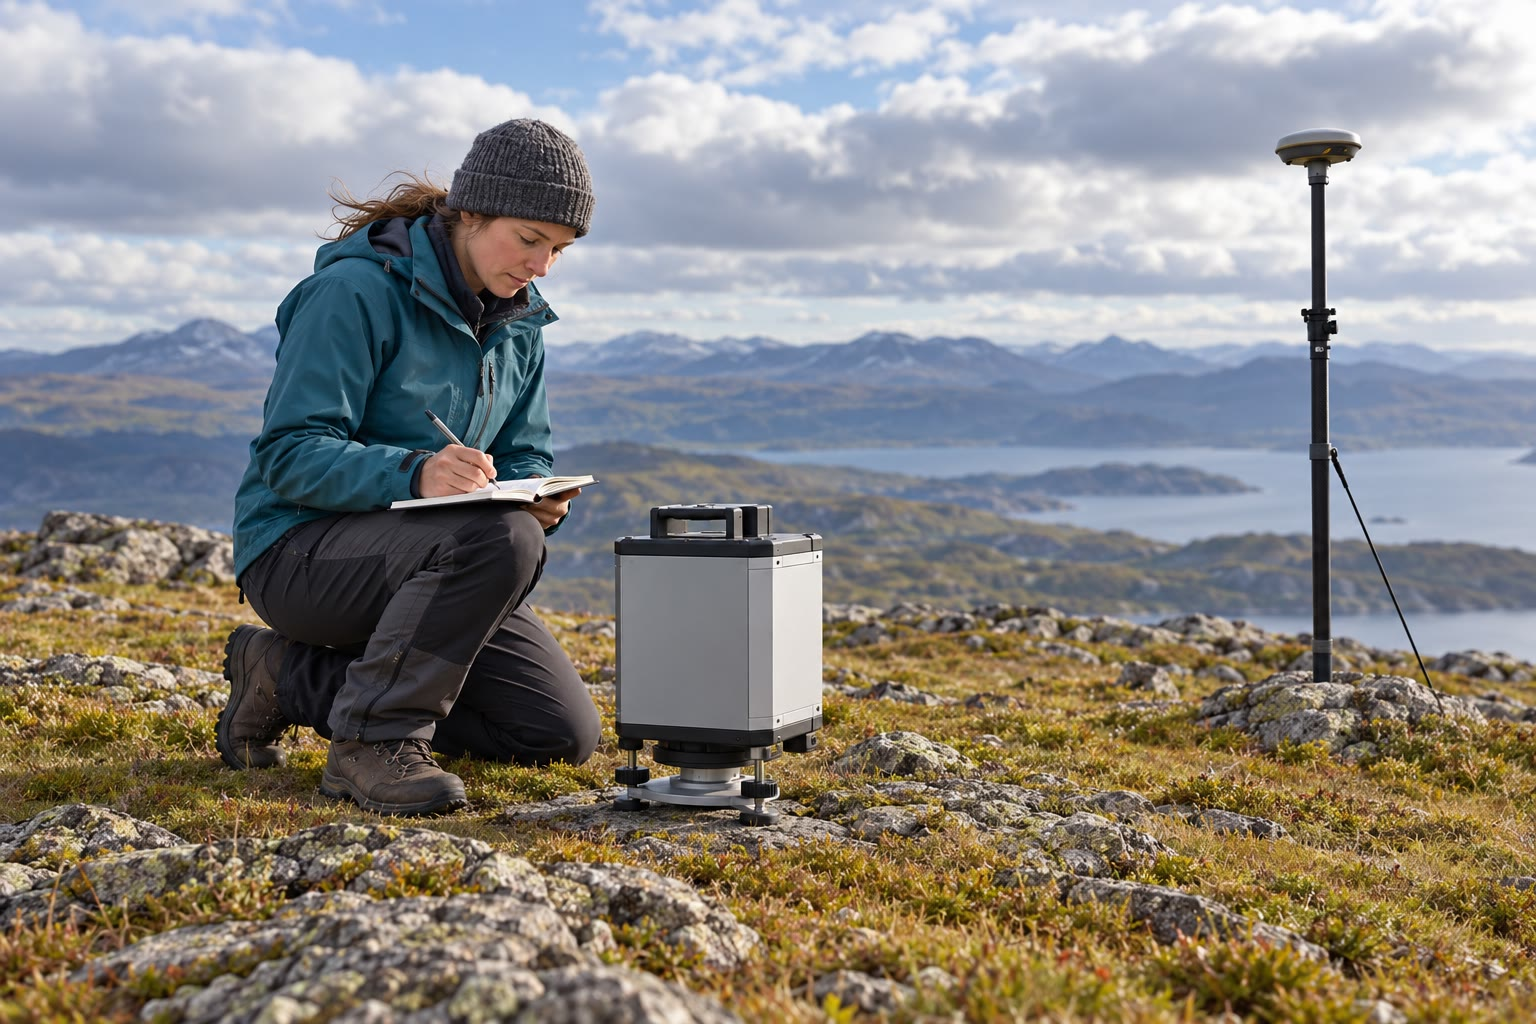
\includegraphics[width=\linewidth]{images/book5/ai/b3-gravimeter.jpg}

{\scriptsize 野外重力仪及其调平底座，背景中为卫星
天线（AI 生成插图）。}
\end{minipage}
\end{inthefield}

\section{练习}

\begin{exercise}[$\star$]\label{exo:b3:gravity-geodesy:1}
由大地测量参考系统 1980 的取值 $a = \qty{6378137}{m}$ 和
$f = \num{0.00335281068}$，求短半轴 $b$ 与 $a - b$。
已知 $J_2 = \num{1.08263e-3}$ 与 $m = \num{0.00344979}$，求克莱罗关系所预言的
扁率，并加以比较。
\end{exercise}

\begin{exercise}[$\star$]\label{exo:b3:gravity-geodesy:2}
在一个干旱年份，一个面积为 \qty{5.0e5}{km^2} 的流域损失了 \qty{60}{Gt} 的
水。求\omterm{def:b3:gravity-geodesy:ewh}{等效水高}的变化。同样的质量会使海平面
上升多少？取每毫米对应 \qty{360}{Gt}。
\end{exercise}

\begin{exercise}[$\star$]\label{exo:b3:gravity-geodesy:3}
利用级数 $\gamma = 9.780327(1 + 0.0053024\sin^2\varphi -
0.0000058\sin^22\varphi)$ \unit{m.s^{-2}}，求赤道、
\ang{45} 处及两极的正常重力。将两极与赤道之差
以毫伽表示。
\end{exercise}

\begin{exercise}[$\star$]\label{exo:b3:gravity-geodesy:4}
求大洋板块的\omterm{def:b3:gravity-geodesy:flexure}{挠曲刚度}与\omterm{def:b3:gravity-geodesy:alpha}{挠曲参数}，取
$T_e = \qty{10}{km}$ 和 $T_e = \qty{30}{km}$（$E = \qty{100}{GPa}$，
$\nu = 0.25$，$\rho_m - \rho_w = \qty{2270}{kg.m^{-3}}$，$g =
\qty{9.81}{m.s^{-2}}$）。在线载荷作用下，环沟边缘与
\omterm{def:b3:gravity-geodesy:alpha}{前缘隆起}分别位于何处？
\end{exercise}

\begin{exercise}[$\star\star$]\label{exo:b3:gravity-geodesy:5}
(a) 若该处大地水准面高为 $+\qty{50}{m}$，求该处的扰动位
（取 $\gamma = \qty{9.80}{m.s^{-2}}$）。(b) 在 \qty{100}{km} 范围内，大地水准面升高
\qty{10}{m}，求该处铅垂线与椭球法线的夹角，
并以角秒表示。
\end{exercise}

\begin{exercise}[$\star\star$]\label{exo:b3:gravity-geodesy:6}
由 $J_2 = \num{1.08263e-3}$ 及转动惯量因子
$C/(Ma^2) = \num{0.3308}$，求动力学椭率 $H = (C - A)/C$ 及
$1/H$。若地球为均匀体且 $J_2$ 相同，两者中哪一个会改变？
\end{exercise}

\begin{exercise}[$\star\star$]\label{exo:b3:gravity-geodesy:7}
一颗卫星在赤道半径之上 \qty{500}{km} 处作圆轨道运行，
（$a = \qty{6378.137}{km}$，$GM = \qty{3.986005e14}{m^3.s^{-2}}$），轨道倾角为
\ang{89}。求其周期及交点进动速率（以度每天计）。
为何重力测量任务多选用近极轨道？
\end{exercise}

\begin{exercise}[$\star\star$]\label{exo:b3:gravity-geodesy:8}
地表两个重力异常均为 \qty{10}{\milli\gal}，其波长分别为
\qty{100}{km} 和 \qty{1000}{km}。求二者在 \qty{500}{km}
高度处的振幅。
\end{exercise}

\begin{exercise}[$\star\star$]\label{exo:b3:gravity-geodesy:9}
在海沟海侧，外隆起顶部距海沟轴线
\qty{120}{km}。取板块上方为水的断裂板块模型，计算
$\alpha$、$D$ 与 $T_e$，并求板块穿过其未挠曲的
水平面处的距离。
\end{exercise}

\begin{exercise}[$\star\star\star$]\label{exo:b3:gravity-geodesy:10}
(a) 验证 $w = w_0e^{-u}(\cos u + \sin u)$，$u = x/\alpha$，满足
$Dw'''' + (\rho_m - \rho_i)gw = 0$，对 $x > 0$ 成立，其中 $\alpha$ 如前定义。
(b) 证明弯矩 $-Dw''$ 在载荷下方最大，
并在 $x = \pi\alpha/4$ 处变号。(c) 板块上表面最可能在何处
开裂，为什么？
\end{exercise}

\begin{exercise}[$\star\star\star$]\label{exo:b3:gravity-geodesy:11}
取 $m = \num{0.00344979}$ 及 $C/(Ma^2) = \num{0.3308}$，反解
达尔文–拉多关系，求静力扁率。与
$f = \num{0.00335281}$ 相比较，求二者之差，以及
赤道高出静力形状的超出高度，并说明这对地幔意味着什么。
\end{exercise}

\begin{exercise}[$\star\star\star$]\label{exo:b3:gravity-geodesy:12}
一颗卫星作圆轨道运行，轨道高度为 \qty{700}{km}，要求全年相对太阳保持相同取向：
其交点须在一个回归年内前进 \ang{360}，
回归年长 \num{365.242}~天。求所需的轨道倾角。
\end{exercise}

\section{问题：奥鲁海岭周围的环沟}

\begin{problem}[{周末问题——地球的形状、火山载荷、
其挠曲环沟及卫星所见的情况}]
\label{pb:b3:gravity-geodesy:1}
% values: calc/ch03.py; GRS80 (geod5:grs80-*), earth:MoI; flexure.py
奥鲁是海洋中虚构的一条火山海岭：由多座相连火山组成的直线状链，
长 \qty{400}{km}，建于古老的大洋岩石圈之上。其截面取为
底宽 \qty{80}{km} 的三角形，
高 \qty{6}{km}，密度为 \qty{2800}{kg.m^{-3}}，立于
水深 \qty{5}{km} 的海底之上。地幔密度 \qty{3300}{kg.m^{-3}}，海水
密度为 \qty{1030}{kg.m^{-3}}，$E = \qty{100}{GPa}$，$\nu = 0.25$，$g =
\qty{9.81}{m.s^{-2}}$，$G = \qty{6.674e-11}{m^3.kg^{-1}.s^{-2}}$。

\medskip
\noindent\textbf{第一部分——地球的形状。} 采用 1980 大地参考系统：
$a = \qty{6378137}{m}$，$b = \qty{6356752.3}{m}$，
$GM = \qty{3.986005e14}{m^3.s^{-2}}$，$J_2 = \num{1.08263e-3}$，
$\omega = \qty{7.292115e-5}{rad.s^{-1}}$，$f = \num{0.00335281}$；以及
$C/(Ma^2) = \num{0.3308}$。
\begin{enumerate}
  \item 计算 $m = \omega^2a^2b/(GM)$。
  \item 由克莱罗关系及 $J_2$ 和 $m$，计算所得扁率
        及其倒数。
  \item 由达尔文–拉多关系计算静力扁率，
        及其倒数。
  \item 将两者与观测扁率比较，赤道高出静力形状的
        高度为多少米？
  \item 计算动力学椭率 $H = (C - A)/C$。
\end{enumerate}

\noindent\textbf{第二部分——载荷。}
\begin{enumerate}[resume]
  \item 计算海岭截面的面积。
  \item 计算线载荷 $V_0$，取整个海岭为没入水中的情形，
        使其单位体积重量为 $(\rho_v - \rho_w)g$。
  \item 若海岭以艾里方式局部补偿，即由其自身岩石在地幔中
        形成一个根，则该根在
        海岭顶部之下的深度为多少？
  \item 若为局部补偿，根将止于海岭坡脚，
        距其轴线 \qty{40}{km}。水深测量显示环沟延伸至
        \qty{165}{km} 处。这说明了什么？
\end{enumerate}

\noindent\textbf{第三部分——挠曲环沟。} 环沟中充满水
（$\rho_i = \rho_w$）。穿过海岭的地震剖面表明，
距轴线 \qty{165}{km} 处洋壳顶面已恢复到区域深度，而
\omterm{def:b3:gravity-geodesy:alpha}{前缘隆起}顶部距轴线 \qty{220}{km}。
\begin{enumerate}[resume]
  \item 由环沟边缘计算\omterm{def:b3:gravity-geodesy:alpha}{挠曲参数}。
  \item 由\omterm{def:b3:gravity-geodesy:alpha}{前缘隆起}再次计算，二者是否一致？
  \item 取 $\alpha = \qty{70.0}{km}$，计算\omterm{def:b3:gravity-geodesy:flexure}{挠曲刚度}。
  \item 计算\omterm{def:b3:gravity-geodesy:flexure}{有效弹性厚度}。
  \item 取 $V_0 = \qty{4.17e12}{N.m^{-1}}$，并将 $D$ 取三位有效数字，
        计算轴线下方的挠度。
  \item 计算\omterm{def:b3:gravity-geodesy:alpha}{前缘隆起}的高度。
  \item 验证整个挠曲的浮力 $2w_0\alpha(\rho_m -
        \rho_w)g$ 与 $V_0$ 相平衡。
  \item 将 $T_e$ 与夏威夷海岭上测得的值比较，为 17 至
        \qty{37}{km}。将轴线下方的挠度与
        第 8 题所得的艾里根相比较。
\end{enumerate}

\noindent\textbf{第四部分——环沟上方的重力。} 取挠曲的一个谐波，
其波长为 $2\pi\alpha$，振幅为 $W = \qty{500}{m}$，同时使
海底（水下地壳密度 \qty{2900}{kg.m^{-3}}，位于海平面以下
\qty{5}{km}）与莫霍面（地壳之下的地幔，位于海平面以下 \qty{12}{km}）。一片
面密度为 $\sigma$ 的薄层紧邻其上方处产生的
重力异常为 $2\pi G\sigma$。
\begin{enumerate}[resume]
  \item 计算该谐波的波长及波数 $k$。
  \item 计算由挠曲海底在海平面处产生的异常振幅，
        由 \qty{5}{km} 深度\omterm{prop:b3:gravity-geodesy:upward}{向上延拓}。
  \item 计算挠曲莫霍面产生的异常振幅及总振幅。
  \item 计算卫星高度处的总异常，该高度位于海平面以上
        \qty{400}{km}。
  \item 波长为 \qty{80}{km}（即海岭宽度）的谐波，在该高度处
        减弱了多少倍？卫星能够分辨什么？
  \item 第 18 题中的谐波对应的球谐阶数 $n \approx 2\pi R/\lambda$
        为多少（取 $R = \qty{6371}{km}$）？
  \item 求出奥鲁海岭之下
        板块的\omterm{def:b3:gravity-geodesy:flexure}{有效弹性厚度}。
\end{enumerate}
\end{problem}
